\chapter{Analysis Diagrams}

\section{Conceptual Framework}

% This is the conceptual framework with career planning.
\makefigure{ht}{
   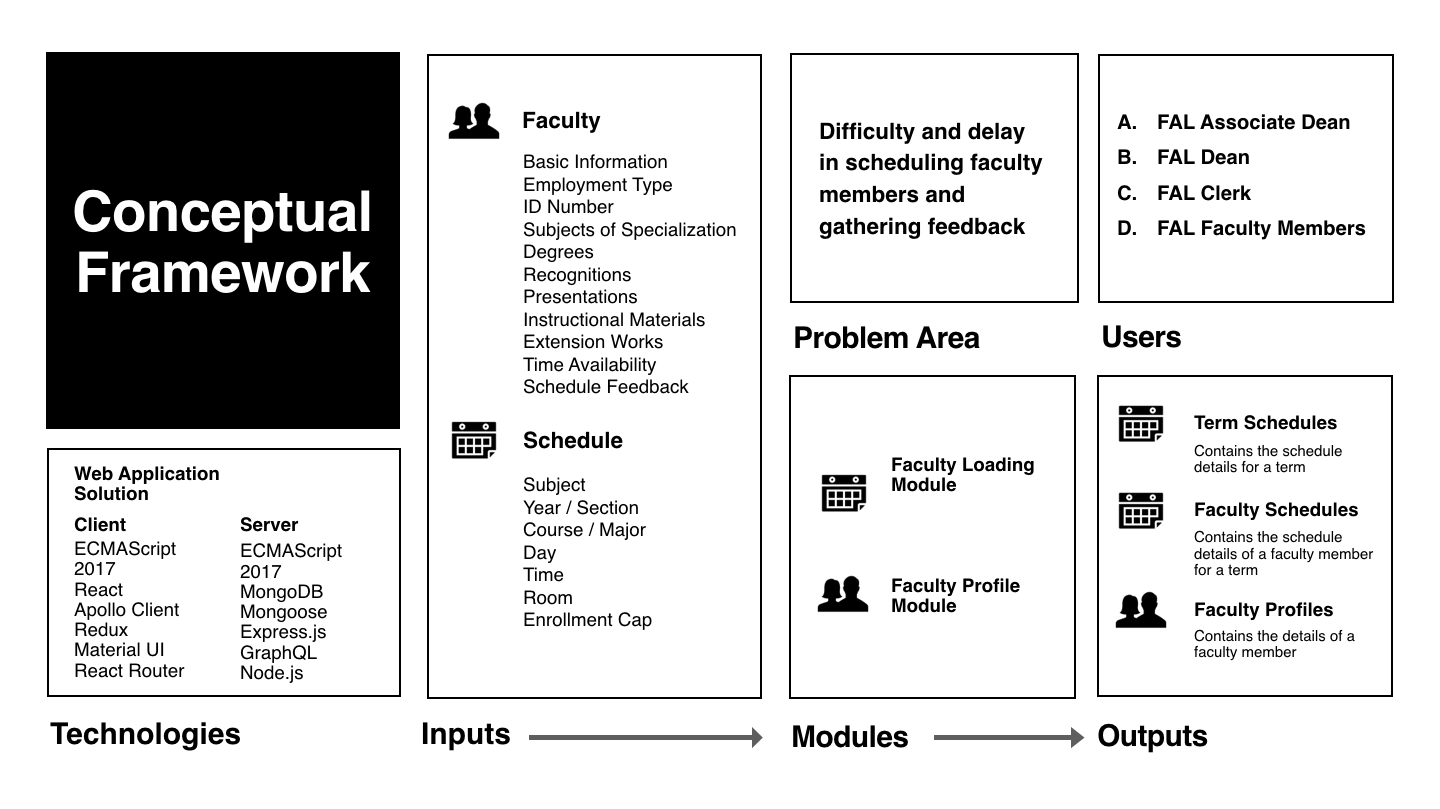
\includegraphics[width=\linewidth]{figures/problem_analysis/Conceptual_Framework.png}
   \caption{The Conceptual Framework}
   \label{appendix:ConceptualFramework}
}

\clearpage

\section{Ishikawa Diagrams}

\makefigure{!ht}{
   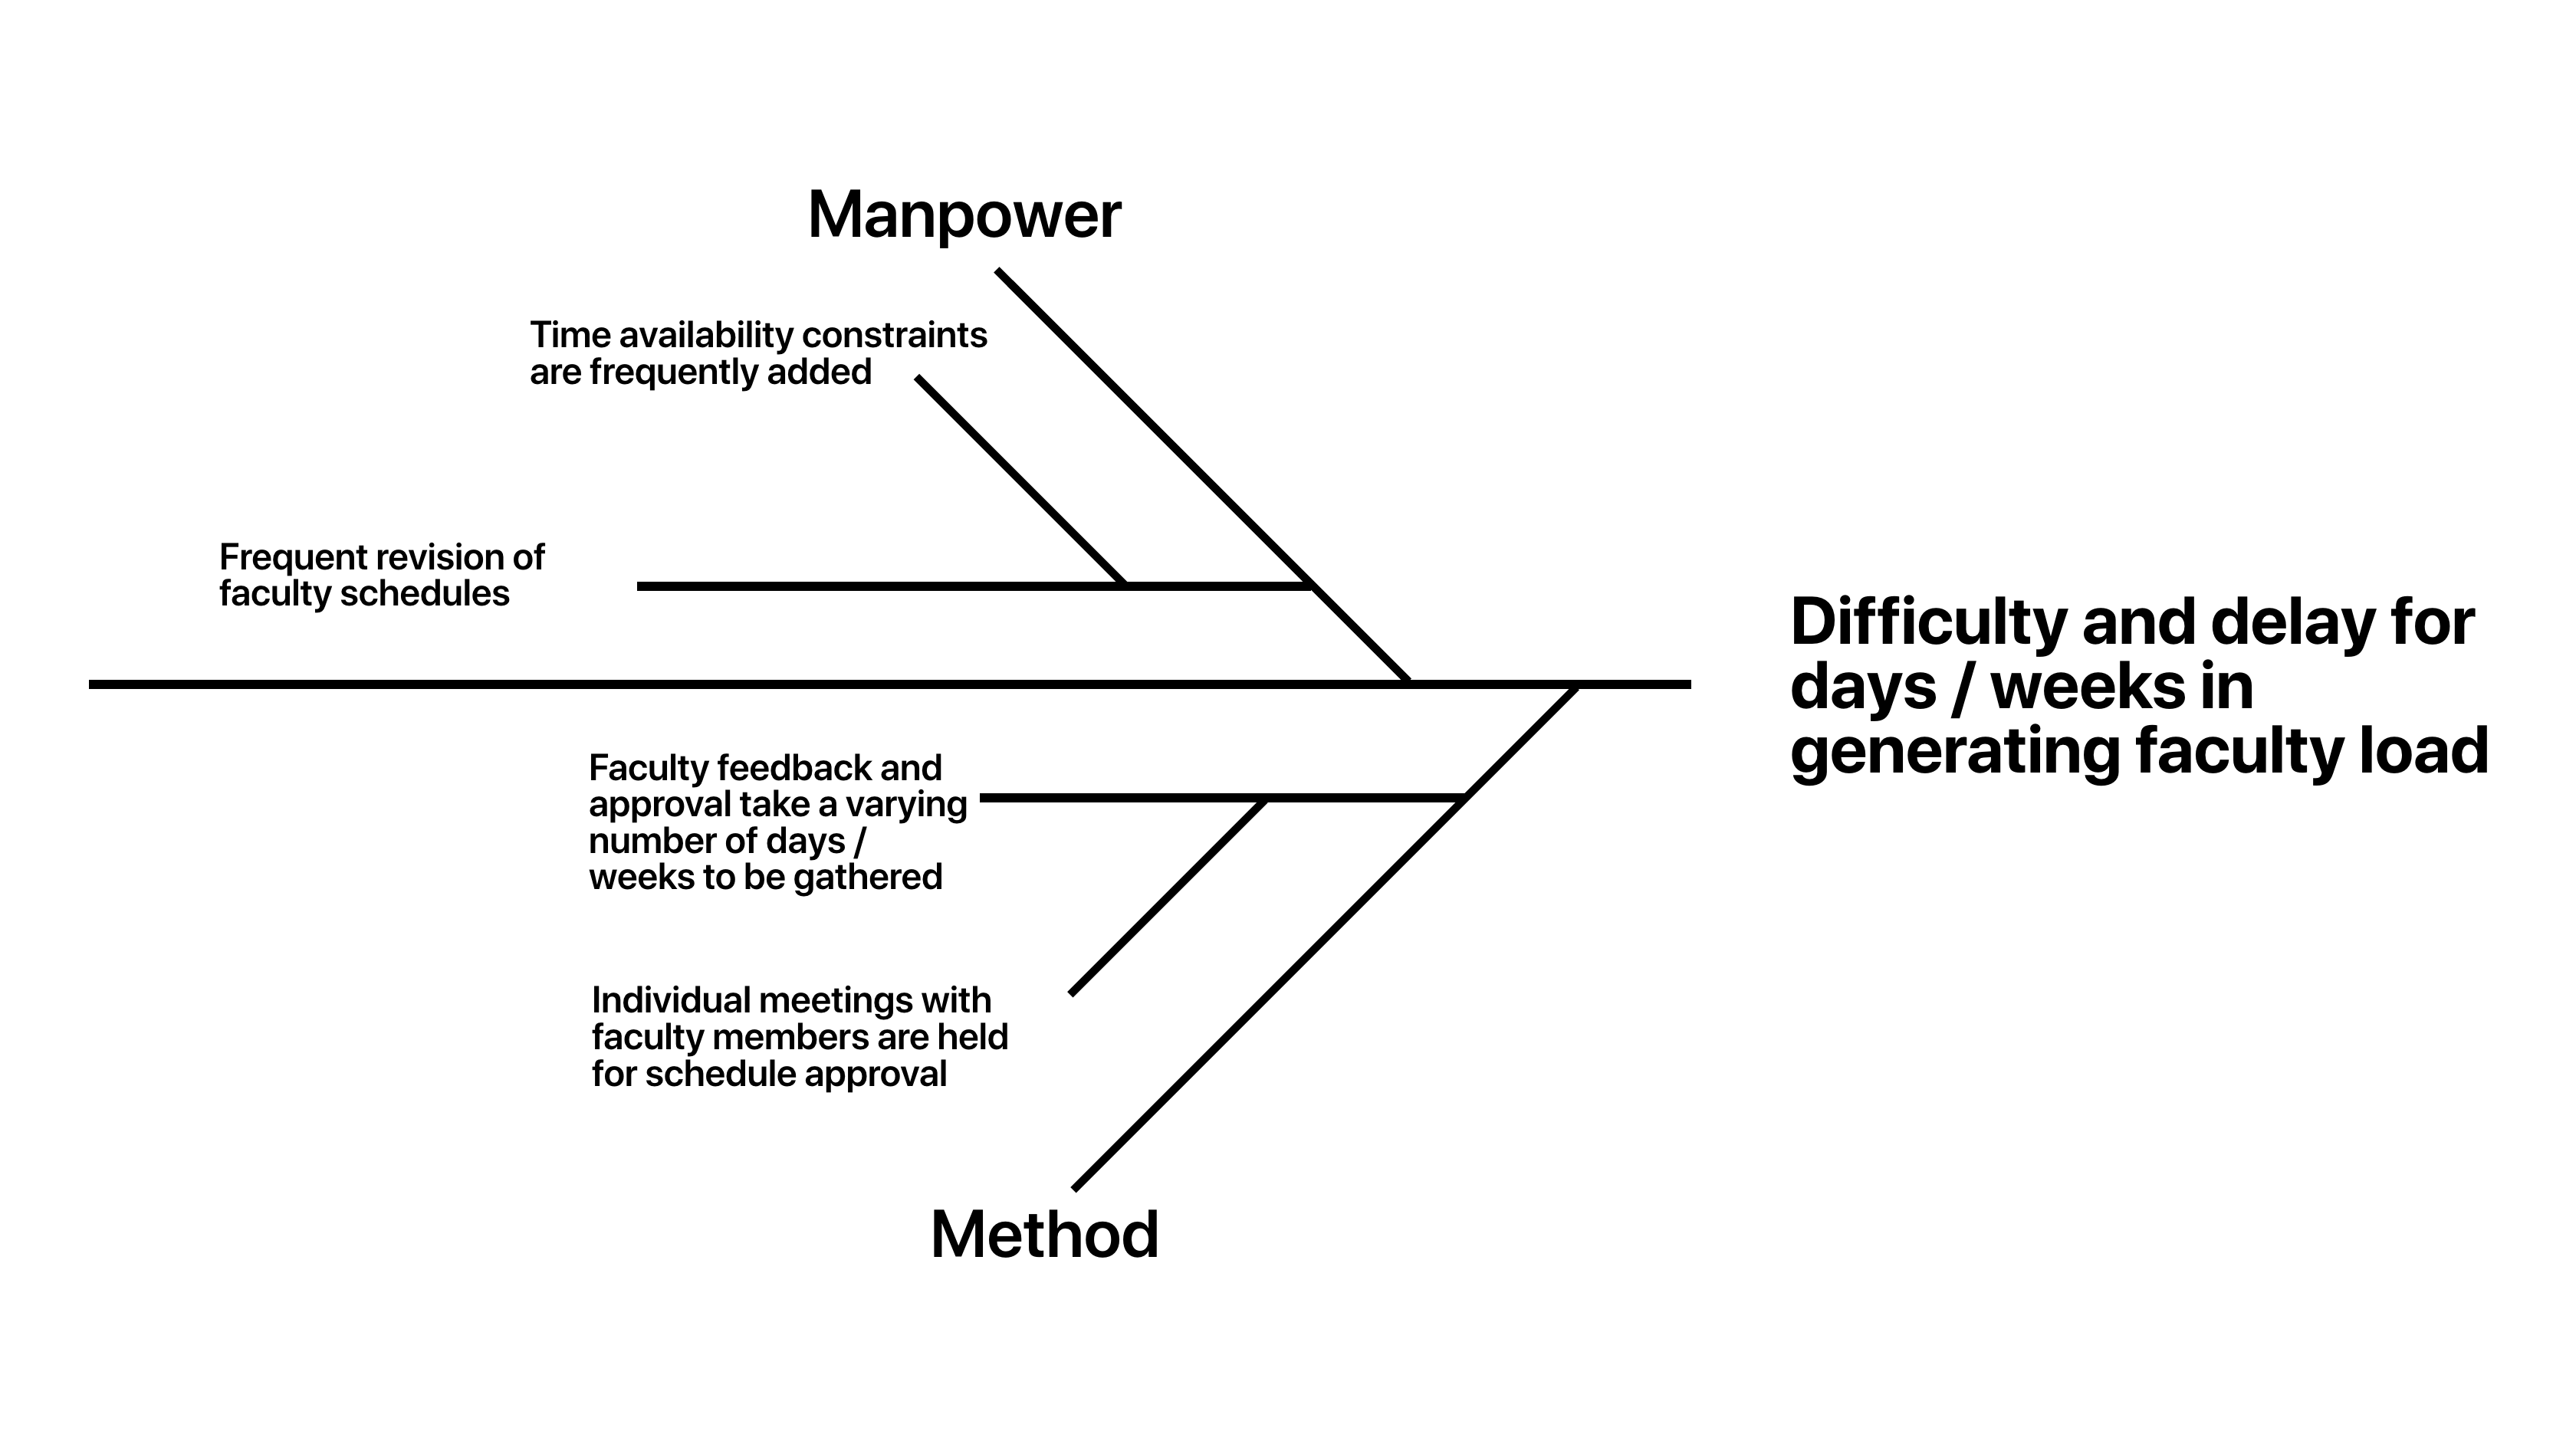
\includegraphics[width=7.5in, angle=90]{figures/problem_analysis/Faculty_Loading_Ishikawa.png}
   \caption{The faculty loading problem analysis}
   \label{appendix:FacultyLoadingIshikawa}
}

\clearpage

\section{Process Diagrams}

\makefigure{ht}{
   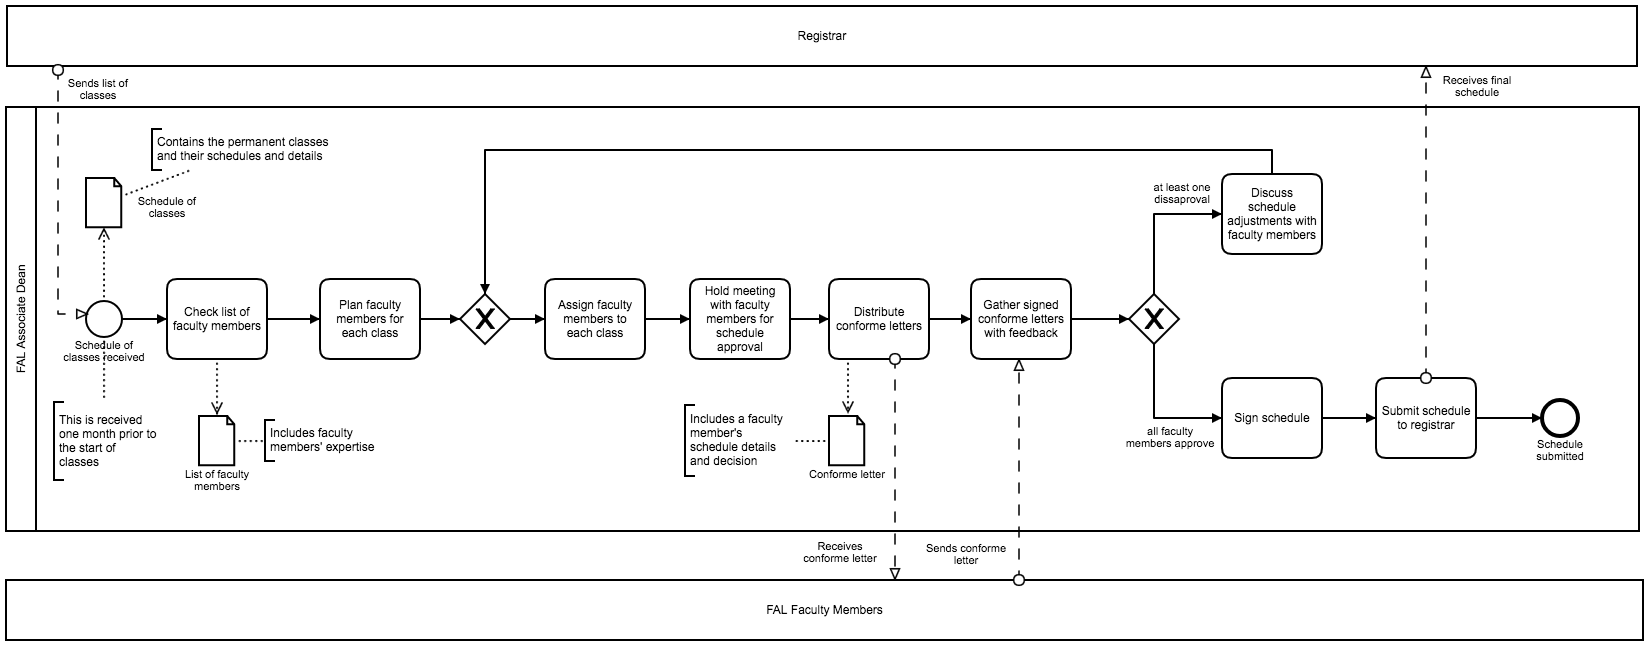
\includegraphics[width=\linewidth, angle=90]{figures/problem_analysis/Current_Faculty_Loading_Process_BPMN.png}
   \caption{The current faculty loading process}
   \label{appendix:FacultyLoadingBPMN}
}

\clearpage

\section{Gantt Chart}

\makefigure{ht}{
   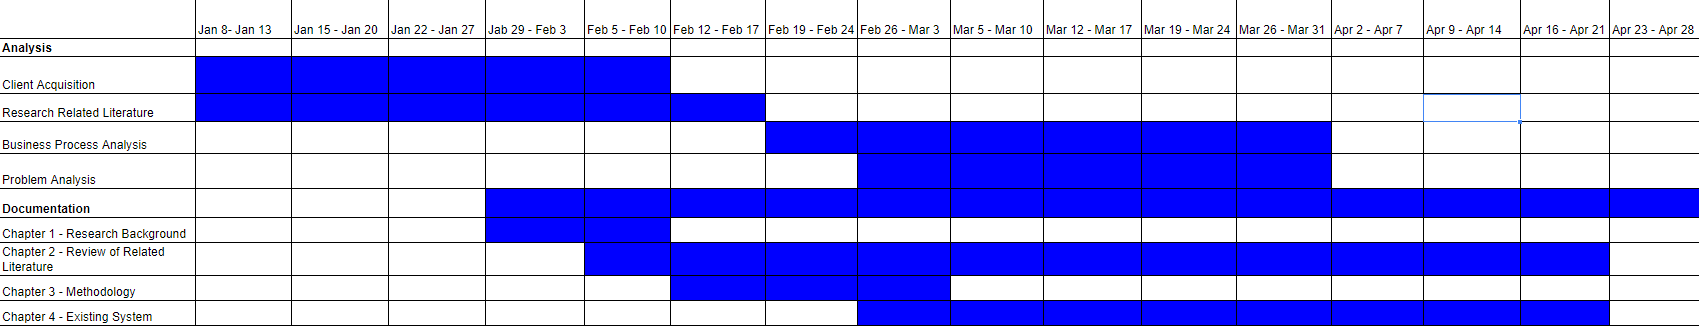
\includegraphics[width=7in, height=2.5in]{figures/problem_analysis/ganttChartAnalysis.png}
   \label{appendix:GanttChart}
}

\makefigure{ht}{
   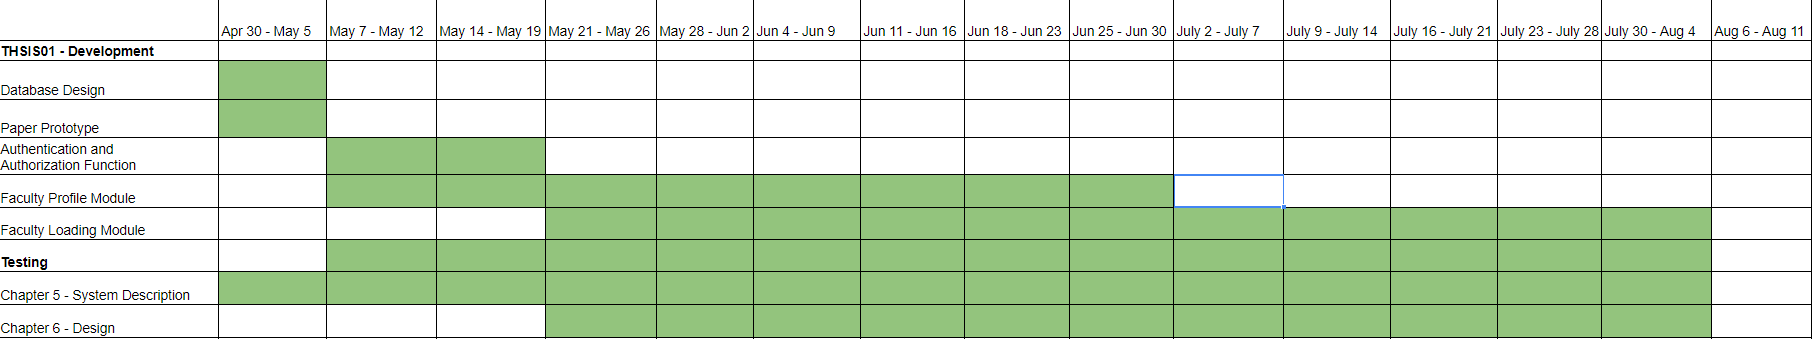
\includegraphics[width=7in, height=2.5in]{figures/problem_analysis/ganttChartThsis1.png}
   \label{appendix:GanttChartThsis1}
}

\makefigure{ht}{
   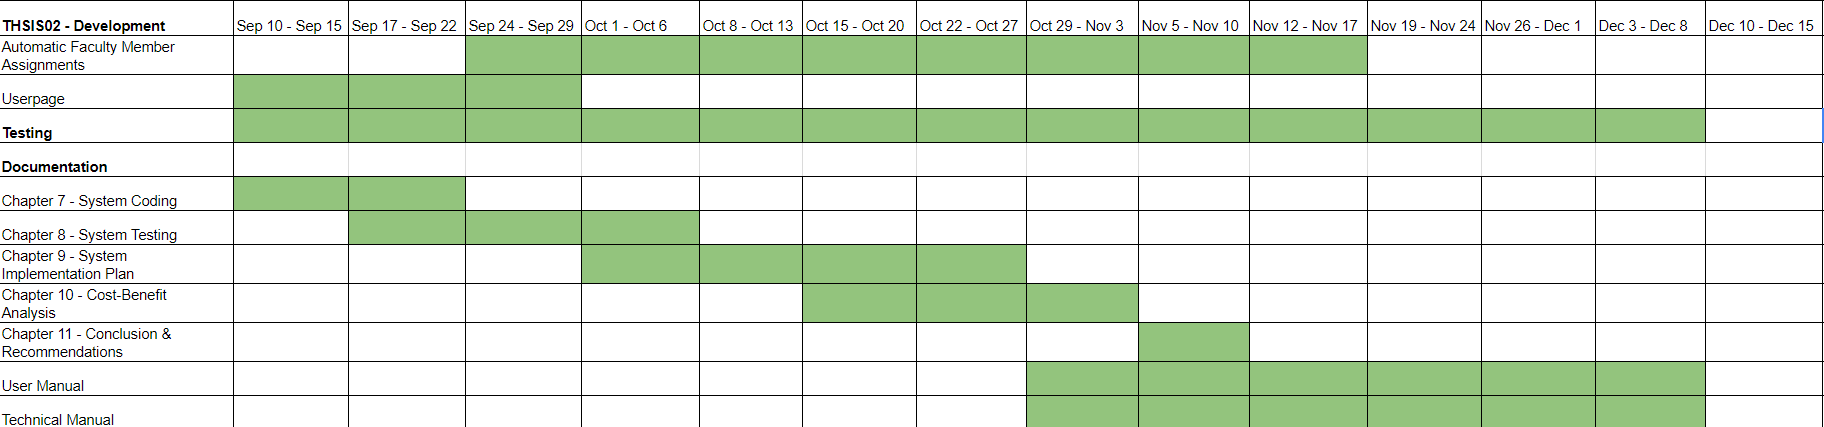
\includegraphics[width=7in, height=2.5in]{figures/problem_analysis/ganttChartThsis2.png}
   \label{appendix:GanttChartThsis2}
}